\documentclass{beamer}

\usepackage[utf8]{inputenc}
\usepackage[russian]{babel}
\usepackage{tikz}
\usepackage{minted}
\usepackage{hyperref}
\usepackage{amssymb}
\usepackage{graphicx}
\usepackage{subcaption}
\usepackage{mathtools} % for :=
\usepackage{movie15}

\usetikzlibrary{shapes,snakes}

\title{D* lite}
\author{Лев Сорвин \\ Максим Хабаров}
\date{2025--01--29}

%\usetheme{Madrid}
\addtobeamertemplate{navigation symbols}{}{%
    \usebeamerfont{footline}%
    \usebeamercolor[fg]{footline}%
    \hspace{1em}%
    \insertframenumber/\inserttotalframenumber
}

\newcommand{\fplan}{\mathtt{plan}}
\newcommand{\fextract}{\mathtt{extract}}
\newcommand{\fempty}{\mathtt{empty}}
\newcommand{\realpositive}{\mathbb{R}_{\geqslant 0}}
\DeclareMathOperator*{\argmin}{arg\,min}




\begin{document}

    \frame{\titlepage}
    \begin{frame}[fragile]
        \frametitle{Мотивация}
        \begin{center}
            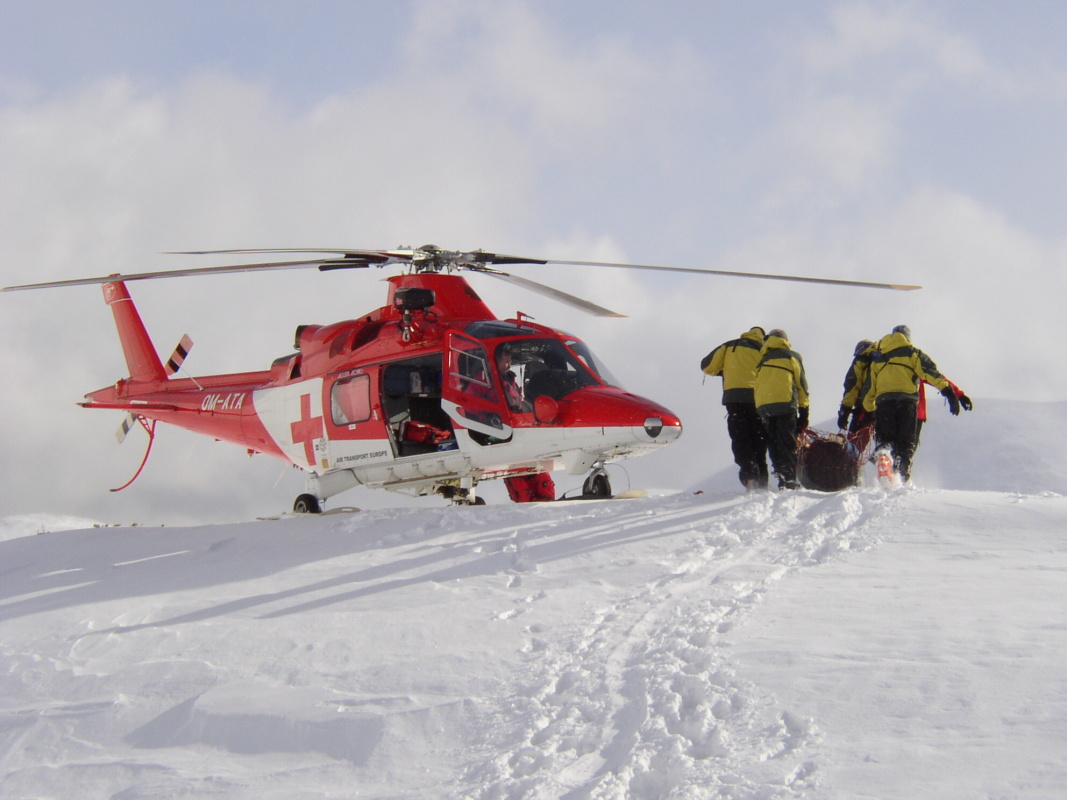
\includegraphics[height=6cm]{../figures/medical-evacuation}
        \end{center}
    \end{frame}

    \begin{frame}[fragile]
        \frametitle{Неформальная постановка задачи}
        \begin{verbatim}
g, start, goal = init_graph()
while undet():
    updates = receive_updated_edges_w()
    replan_shortest_path( # LPA*
        start,
        goal,
        g,
        updates,
        h)
# нет шага step
        \end{verbatim}
    \end{frame}

    \begin{frame}[fragile]
        \frametitle{Постановка задачи -- обозначения}
        $G = (V, E)$ -- граф; $V$ --- конечное множество вершин, $E \subset V \times V \times \realpositive$ --- взвешенные ребра.

        $w: V \times V \rightarrow {\realpositive \lor \infty}$ -- функция веса ребра.

        $A = [v_1, v_2, \dots, v_n]: \forall i = 1, \dots, n-1$: $w(v_i, v_{i+1}) \neq \infty$  --- путь в графе.

        $P = P(V)$ --- множество путей в графе.

        $w(A) = \sum_{i = 1}^{n-1} w(v_i, v_{i+1})$ --- вес пути.

        $s(A)$ --- начало пути, $d(A)$ --- конец пути.

    \end{frame}

    \begin{frame}[fragile]
        \frametitle{Формальная математическая постановка задачи}

        Задача минимального пути --- нам даны вершины $s, d \in V$  (далее мы считаем, что $s, d, V$ фиксированы) и мы должны найти
        $$A_{plan}= \argmin_{\substack{A \subset V \text{ --- путь в } G \\ s(A) = s \\ d(A) = d}} w(A).$$
        Мы будем также говорить тогда, что $A = \mathtt{optpath}(G, s, d)$.

    \end{frame}

    \begin{frame}[fragile]
        \frametitle{Формальная алгоритмическая постановка задачи}

        Мы хотим решать задачу минимального пути \textit{онлайн} (longterm planning).
        Ее решение --- тройка $(T, \fplan, \fextract)$ из произвольного множества и двух вычислимых фукнций соответственно, такую что:
        \begin{align*}
            &\fempty \in T \\
            &\fplan: E \times T \rightarrow T \\
            &\fextract: T \rightarrow P(V) \\
            &\fextract(\fplan(E, \fempty)) = \mathtt{optpath}(G, s, d) \\
            &\fextract(t_0) = \mathtt{optpath}((V, E'), s, d) \rightarrow \\
            &\qquad \fextract(\fplan(E_{new}, t_0)) = \mathtt{optpath}((V, E' \leftarrow E_{new}), s, d)
        \end{align*}

    \end{frame}


    \begin{frame}
        \frametitle{Известные решения}
        \begin{itemize}
            \item Повторный A* на новых весах
            \item Dynamic SWSF-FP
            \begin{itemize}
                \item Переиспользует предыдущие результаты поиска
                \item $\approx$ BFS
            \end{itemize}
        \end{itemize}
    \end{frame}

    \begin{frame}
        \frametitle{Пересчет}
        \begin{figure}
            \centering
            \begin{subfigure}[b]{0.49\textwidth}
                \centering
                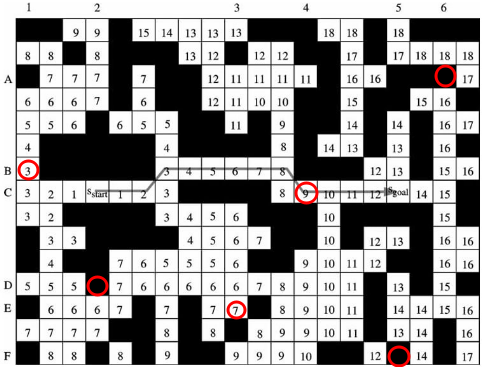
\includegraphics[width=\textwidth]{../figures/before-block.png}
            \end{subfigure}
            \hfill
            \begin{subfigure}[b]{0.49\textwidth}
                \centering
                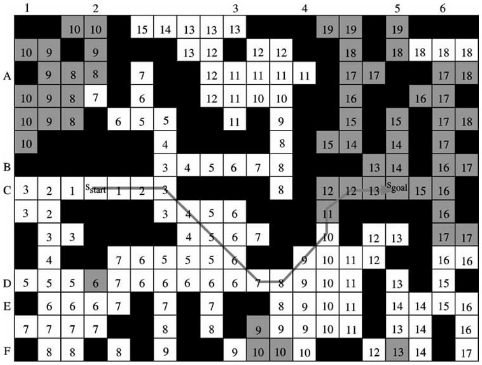
\includegraphics[width=\textwidth]{../figures/after-block.png}
            \end{subfigure}
        \end{figure}

    \end{frame}

    \begin{frame}
        \frametitle{Алгоритм LPA* --- идея}

        \begin{align*}
            &g^*(v) = \begin{cases}
                          0 &  v = s\\
                          \displaystyle \min_{v' \in neighbors(v)} (w(v, v') + g^*(v')) \\
            \end{cases} \\
            &rhs(v) \coloneq \min_{v' \in neighbors(v)} (w(v, v') + g(v')) \\ \\
            &rhs(v) = g(v)\ \forall v \in V \leftrightarrow g(v) = g^*(v)
        \end{align*}
        \begin{itemize}
            \item $rhs(v) \neq g(v)$ --- локальная неконсистентность
        \end{itemize}


    \end{frame}
    \begin{frame}[fragile]
        \frametitle{Алгоритм D* lite}
        \begin{center}
            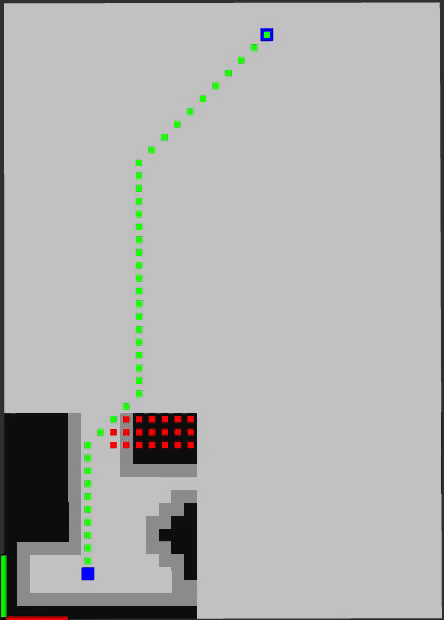
\includegraphics[height=.75\textheight]{../figures/dstar8cells}
        \end{center}

    \end{frame}

    \begin{frame}
        \frametitle{План экспериментов}
        \begin{itemize}
            \item Сравнить:
            \begin{itemize}
                \item Повторную A*
                \item DynamicSWSF-FP
                \item D* llite
            \end{itemize}
            \item На:
            \begin{itemize}
                \item Лабиринте
                \item Помещении
                \item Улице
            \end{itemize}
            \item Детали:
            \begin{itemize}
                \item Кардинальные ходы
                \item Датасет MovingAI
            \end{itemize}
        \end{itemize}
    \end{frame}

    \begin{frame}
        \frametitle{Графики при малой видимости}
        \begin{figure}
            \centering
            \begin{subfigure}[b]{0.49\textwidth}
                \centering
                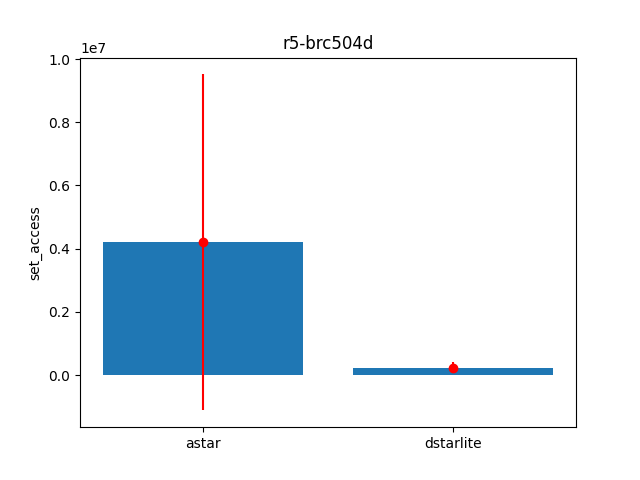
\includegraphics[width=\textwidth]{../figures/astar-to-dstarlite/r5-brc504d}
            \end{subfigure}
            \hfill
            \begin{subfigure}[b]{0.49\textwidth}
                \centering
                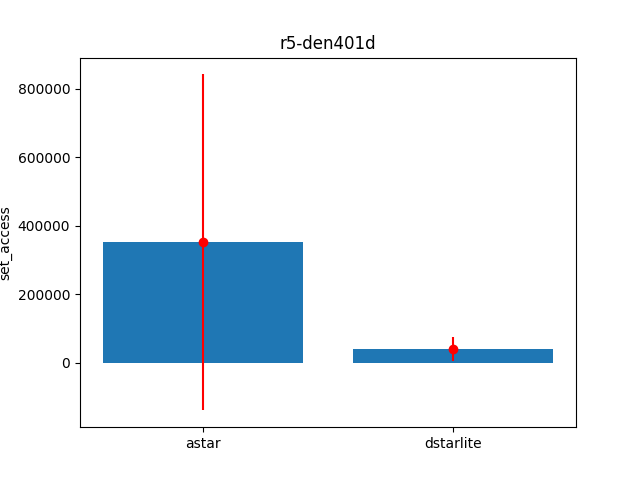
\includegraphics[width=\textwidth]{../figures/astar-to-dstarlite/r5-den401d}
            \end{subfigure}
            \hfill
            \begin{subfigure}[b]{0.49\textwidth}
                \centering
                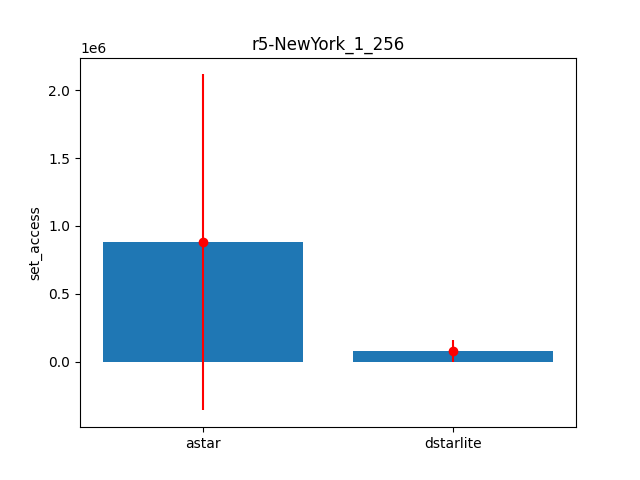
\includegraphics[width=\textwidth]{../figures/astar-to-dstarlite/r5-NewYork_1_256}
            \end{subfigure}
            \hfill
            \begin{subfigure}[b]{0.49\textwidth}
                \centering
                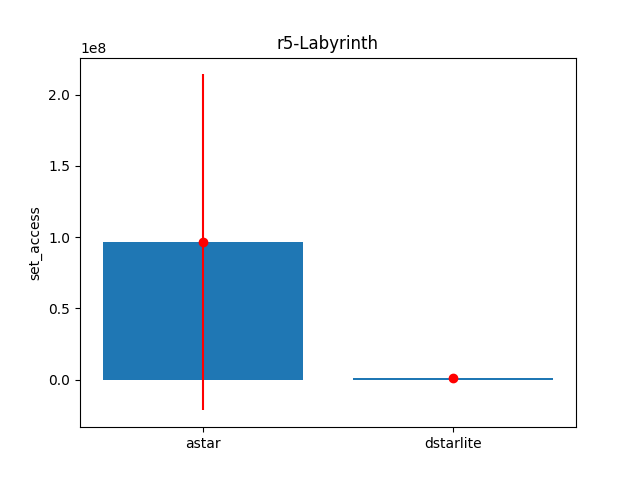
\includegraphics[width=\textwidth]{../figures/astar-to-dstarlite/r5-Labyrinth}
            \end{subfigure}
        \end{figure}
    \end{frame}

    \begin{frame}
        \frametitle{Графики при большой видимости}
        \begin{figure}
            \centering
            \begin{subfigure}[b]{0.49\textwidth}
                \centering
                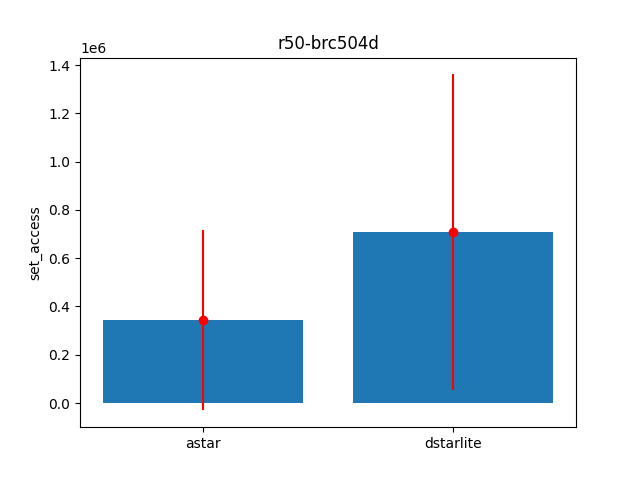
\includegraphics[width=\textwidth]{../figures/astar-to-dstarlite/r50-brc504d}
            \end{subfigure}
            \hfill
            \begin{subfigure}[b]{0.49\textwidth}
                \centering
                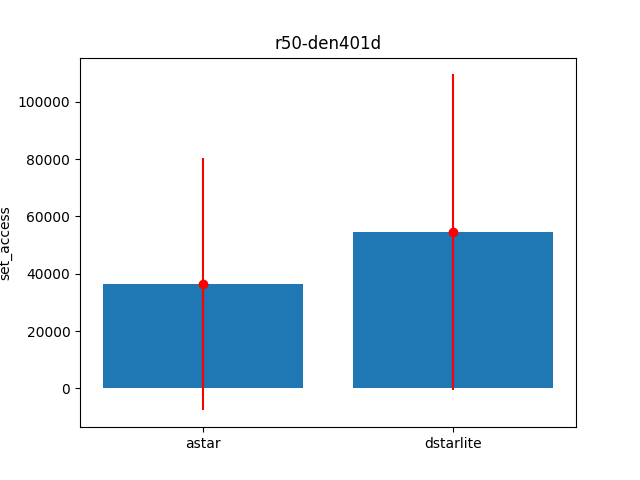
\includegraphics[width=\textwidth]{../figures/astar-to-dstarlite/r50-den401d}
            \end{subfigure}
            \hfill
            \begin{subfigure}[b]{0.49\textwidth}
                \centering
                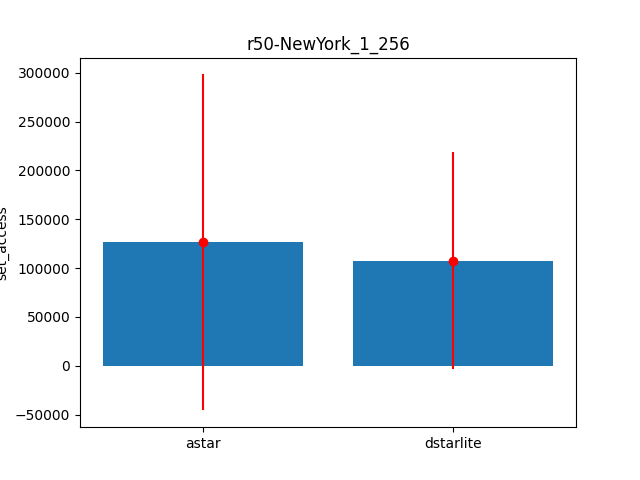
\includegraphics[width=\textwidth]{../figures/astar-to-dstarlite/r50-NewYork_1_256}
            \end{subfigure}
            \hfill
            \begin{subfigure}[b]{0.49\textwidth}
                \centering
                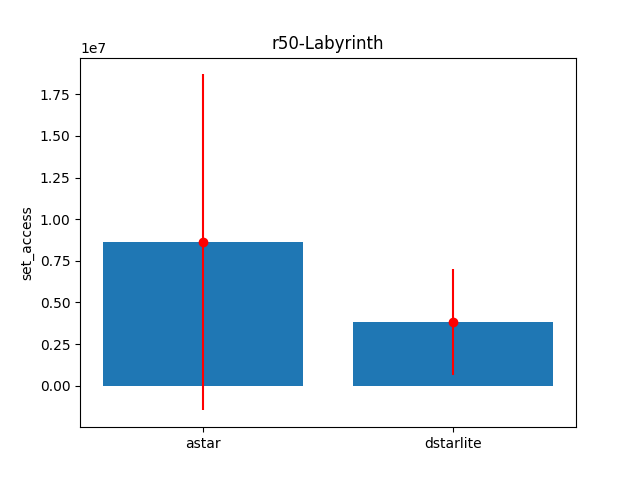
\includegraphics[width=\textwidth]{../figures/astar-to-dstarlite/r50-Labyrinth}
            \end{subfigure}
        \end{figure}
    \end{frame}


    \begin{frame}
        \frametitle{Результаты производительности (мс)}
        Низкая видимость (радиус 5)

        \begin{tabular}{lllll}
            \hline
            & brc504d     & den401d     & NewYork     & Labyrinth   \\
            \hline
            swsffp  & 1.4e4±3.2e4 & 4.9e2±7.3e2 & 1.1e3±2.8e3 & NA          \\
            a*      & 5.8e2±1.5e3 & 5.2e1±1.5e2 & 1.5e2±4.6e2 & 2.3e4±6.1e4 \\
            d* lite & 3.3e2±4.7e2 & 5.8e1±8.6e1 & 1.3e2±2.3e2 & 3.0e3±4.6e3 \\
            \hline
        \end{tabular}

        \bigskip
        Высокая видимость (радиус 50)

        \begin{tabular}{lllll}
            \hline
            & brc504d     & den401d     & NewYork     & Labyrinth   \\
            \hline
            swsffp & 1.4e4±2.3e4 & 8.6e2±1.1e3 & 2.5e3±3.4e3 & NA          \\
            astar  & 6.9e1±1.3e2 & 1.2e1±2.1e1 & 3.1e1±7.5e1 & 2.2e3±5.4e3 \\
            d*     & 1.0e3±1.8e3 & 1.1e2±1.6e2 & 1.9e2±3.2e2 & 7.9e3±1.2e4 \\
            \hline
        \end{tabular}

    \end{frame}

    \newcommand{\dstarlite}{\(D^*\ lite\)\,}
    \begin{frame}
        \frametitle{Заключение}
    \end{frame}
\end{document}


